\documentclass[journal]{IEEEtran}
\usepackage{color}
\usepackage{cite}
\usepackage{multirow}
\usepackage{float}
\usepackage{amsfonts}
\usepackage{amssymb}
\usepackage{amsmath}
\usepackage{amsthm}
\usepackage{url}
\usepackage{enumitem}
\usepackage{array}
\usepackage{booktabs}
\usepackage[utf8]{inputenc}
\usepackage[english]{babel}
\usepackage{algorithm}
\usepackage[noend]{algpseudocode}
\usepackage{tikz}
\usetikzlibrary{positioning,arrows}

\newtheorem{definition}{Definition}
\newtheorem{constraint}{Constraint}
\newtheorem{assumption}{Assumption}
\newtheorem{law}{Law}
\newtheorem{invariant}{Invariant}
\newtheorem{proposition}{Proposition}
\newtheorem{obligation}{Obligation}

\author{Ryan~J.~Kung%
\thanks{Ryan J. Kung can be reached at ryankung@ieee.org.
Manuscript created February 11, 2023; rewritten August 31, 2026;
revised September 1, 2026.
This document supersedes the 2023 draft \emph{The Ranking Protocol}.}}
\title{\huge The DRanking Protocol:\\
Verifiable Distributed Ranking and Sybil-Bounded Admission\\
for Structured Peer-to-Peer Networks}
\date{}

\IEEEaftertitletext{%
\vspace{0.5\baselineskip}%
\noindent\hfill
\parbox{0.90\textwidth}{%
\centering\bfseries Abstract\\[0.5\baselineskip]%
\normalfont
DRanking converts locally observed peer behavior in an open structured
peer-to-peer network into a globally agreed, verifiable service weight that
gates admission to protocol roles.  Identity creation is free, so no
mechanism bounds adversarial \emph{count}~\cite{Douceur2002}; the protocol
instead bounds adversarial \emph{weight} and prices it.  The instruments
are: counterparty-signed service receipts in place of unsigned counters; a
seed-anchored trust flow
$t_{k+1}=\alpha C_k^{\mathsf T}t_k+(1-\alpha)s$
obeying conservation, attenuation, and revocation laws, with a proved bound
$T_k(A)\le\alpha g/(1-\alpha)$ on Sybil mass; trust-weighted verifiable
random sortition in place of oracle sampling; a proof-of-authority ledger
trusted for ordering only, with equivocation proofs as first-class slash
objects; and a circuit-friendly epoch transition folded by Nova-family
incrementally verifiable computation, giving constant-cost verification to
browser nodes.  Rank is soulbound and slashable; reward is a separate
transferable asset; the authority-to-stake transition is conditioned on a
security-budget crossover.}}

\begin{document}
\maketitle

\section{Introduction}

The 2023 draft of this protocol scored behavior per identity.  Identities
are free; every component secured against lying nodes fell to numerous
nodes.  This rewrite keeps the draft's decomposition --- local evidence,
global aggregation, sampling, ledger, incentives --- and replaces the
quantity being secured:

\[
\begin{array}{rcl}
\mathsf{cost}(\mathsf{did})&=&0,\\
|\mathsf{Adv}\cap V|&\leq&\infty,\\
\mathsf{secure}(|\cdot|)&=&\bot\quad\text{\cite{Douceur2002}},\\[2pt]
\mathsf{secure}&:=&\mathsf{secure}(T(\cdot)),\\
T(A)&=&\textstyle\sum_{v\in A}t(v),\\
\mathsf{claim}&=&\mathsf{price}\bigl(T(\mathsf{Adv})\geq\tfrac13\bigr).
\end{array}
\]

Sections~\ref{sec:model}--\ref{sec:economics} construct $t$, its evidence,
its sampling, its ledger, and its economy; Section~\ref{sec:security}
tabulates the attack surface.  Each mechanism is a term of
$\mathsf{price}$.

\section{Model}\label{sec:model}

\begin{definition}[Substrate]\label{def:substrate}
\[
\begin{array}{rcl}
R&=&\mathbb{Z}/2^{160}\mathbb{Z}\quad\text{\cite{Chord,ZaveChordCorrect}},\\
\mathsf{did}&:&K\to R,\quad\text{self-certifying},\\
\mathsf{link}&\subseteq&V\times V,\quad\text{authenticated},\\
\mathsf{msg}&=&\langle m,\sigma_{\mathsf{origin}}\rangle,\\
\mathsf{cost}(\mathsf{did})&=&0,\\
\mathsf{cost}(\mathsf{link})&=&\varepsilon>0.
\end{array}
\]
\end{definition}

\begin{definition}[Epoch]
\[
k\in\mathbb{N},\qquad
\mathsf{epoch}(k)=[\,\mathsf{fin}(\Sigma_k),\ \mathsf{fin}(\Sigma_{k+1})\,),
\]
delimited by ledger finality (Definition~\ref{def:ledger}).
\end{definition}

\begin{assumption}[Adversary]\label{asm:adversary}
\[
\begin{array}{rcl}
|\mathsf{Adv}|&\leq&\infty,\\
\mathsf{collude},\ \mathsf{grind},\ \mathsf{patience}&\in&
  \mathsf{Cap}(\mathsf{Adv}),\\
\mathsf{byzantine}&\in&\mathsf{Cap}(\mathsf{Adv}),\\
\mathsf{forge}(\sigma_h),\ h\notin\mathsf{Adv}&\notin&
  \mathsf{Cap}(\mathsf{Adv}),\\
\mathsf{break}(\mathsf{VRF})&\notin&\mathsf{Cap}(\mathsf{Adv}).
\end{array}
\]
\end{assumption}

\begin{assumption}[Honest weight]\label{asm:honest-weight}
\[
T_k(\mathsf{Adv})\;<\;\tfrac13\,T_k(V)\qquad\forall k.
\]
No bound is assumed on $|\mathsf{Adv}|$.
\end{assumption}

\begin{figure}[htbp]
\centering
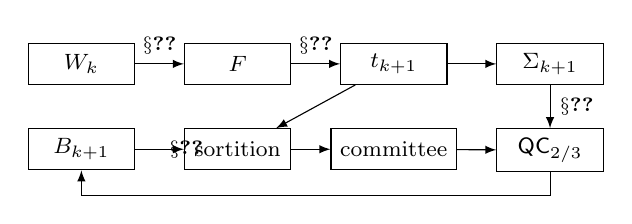
\begin{tikzpicture}[>=latex,
  box/.style={draw,minimum width=1.35cm,minimum height=.52cm,
    align=center,font=\footnotesize}]
\node[box] (w) {$W_k$};
\node[box,right=0.62cm of w] (f) {$F$};
\node[box,right=0.62cm of f] (t) {$t_{k+1}$};
\node[box,right=0.62cm of t] (sig) {$\Sigma_{k+1}$};
\node[box,below=0.55cm of sig] (qc) {$\mathsf{QC}_{2/3}$};
\node[box,below=0.55cm of t] (com) {committee};
\node[box,below=0.55cm of f] (sor) {sortition};
\node[box,below=0.55cm of w] (b) {$B_{k+1}$};
\draw[->] (w) -- node[above,font=\scriptsize]{$\S\ref{sec:receipts}$} (f);
\draw[->] (f) -- node[above,font=\scriptsize]{$\S\ref{sec:trust}$} (t);
\draw[->] (t) -- (sig);
\draw[->] (sig) -- node[right,font=\scriptsize]{$\S\ref{sec:ledger}$} (qc);
\draw[->] (qc.south) -- ++(0,-0.3) -| (b.south);
\draw[->] (b) -- node[right,font=\scriptsize]{$\S\ref{sec:sampling}$} (sor);
\draw[->] (sor) -- (com);
\draw[->] (com) -- (qc);
\draw[->] (t) -- (sor);
\end{tikzpicture}
\caption{Epoch cycle: receipts fold into trust, trust seats the
committee, the committee finalizes the ledger, finality seeds the beacon.}
\label{fig:cycle}
\end{figure}

\section{Service Receipts}\label{sec:receipts}

Unsigned counters are first-person testimony; aggregated, they are hearsay.
The unit of evidence is a countersigned receipt.

\begin{definition}[Receipt]\label{def:receipt}
\[
\rho=\langle\mathsf{srv},a,b,k,n,\sigma_b\rangle,
\]
\[
\begin{array}{rcl}
\mathsf{srv}&\in&\{\mathsf{relay},\mathsf{store},\mathsf{probe}\},\\
a&=&\text{server},\quad b=\text{signer/served},\\
\mathsf{valid}(\rho)&\equiv&
  \mathsf{Vrfy}(k_b,\sigma_b,\mathsf{srv}\Vert a\Vert b\Vert k\Vert n)=\top\\
&&\land\ (b,k,n)\ \text{fresh}.
\end{array}
\]
\end{definition}

\begin{proposition}[Forgery surface]\label{prop:forgery}
\[
\mathsf{valid}(\rho)\land b\notin\mathsf{Adv}
\;\Rightarrow\;
\rho\ \text{issued by}\ b.
\]
\begin{proof}
Immediate from
$\mathsf{forge}(\sigma_b)\notin\mathsf{Cap}(\mathsf{Adv})$
(Assumption~\ref{asm:adversary}).  Manufacturable receipts are exactly
those with $b\in\mathsf{Adv}$ (self-dealing); these are neutralized by
signer-trust weighting (Section~\ref{sec:trust}).
\end{proof}
\end{proposition}

\begin{definition}[Receipt graph]\label{def:graph}
\[
\begin{array}{rcl}
\mathsf{val}(\rho)&=&\mu_{\mathsf{srv}(\rho)}\cdot
  \mathsf{units}(\rho),\quad\mu\ \text{published per kind},\\
W_k&\in&\mathbb{R}_{\geq0}^{V\times V},\\
W_k[b,a]&=&\textstyle\sum\{\mathsf{val}(\rho):
  \rho\ \text{valid},\ \mathsf{sig}\ b,\ \mathsf{srv}\ a,\ \mathsf{ep}\ k\},\\
W_k[b,\cdot]\,\mathbf{1}&\leq&w_{\max}.
\end{array}
\]
\end{definition}

The cap makes countersigning a budgeted act; the protocol certifies
performed service, never synthetic load
(cf.\ Constraint~\ref{con:anchors}).

\section{Trust Algebra}\label{sec:trust}

\begin{definition}[Seed vector]\label{def:seed}
\[
\begin{array}{rcl}
s&\in&[0,1]^{V},\qquad
\textstyle\sum_v s_v=1,\\
\mathsf{supp}(s)&=&S\quad\text{(authority set)}.
\end{array}
\]
\end{definition}

\begin{law}[Conservation]\label{law:conservation}
\[
C_k[b,a]=\frac{W_k[b,a]}{\max\bigl(w_{\max},\ W_k[b,\cdot]\,\mathbf{1}\bigr)},
\qquad
C_k[b,\cdot]\,\mathbf{1}\leq1.
\]
\end{law}

\begin{law}[Attenuation]\label{law:attenuation}
\[
\alpha\in(0,1),\qquad
\mathsf{flow}(\ell\ \text{hops})\leq\alpha^{\ell}.
\]
\end{law}

\begin{law}[Revocation]\label{law:revocation}
\[
\begin{array}{rcl}
\mathsf{slash}(v)&\Rightarrow&t(v):=0,\ v\notin\mathsf{carrier}(t),\\
t_{k+1}&=&f(W_k,t_k)\quad\text{(re-derived per epoch)},\\
s&&\text{withdrawable per seed}.
\end{array}
\]
\end{law}

\begin{definition}[Trust update]\label{def:update}
\begin{equation}\label{eq:update}
t_{k+1}=\alpha\,C_k^{\mathsf T}t_k+(1-\alpha)\,s .
\end{equation}
One power-iteration step per epoch toward
$t^{*}=(1-\alpha)(I-\alpha C^{\mathsf T})^{-1}s$
\cite{PageRank,EigenTrust}; the fixpoint is approached along chain time,
never computed within an epoch (cf.\ Definition~\ref{def:step}).
\end{definition}

\begin{invariant}[Mass]\label{inv:mass}
\[
\textstyle\sum_v t_0(v)=1
\;\Rightarrow\;
\textstyle\sum_v t_k(v)\leq1\quad\forall k.
\]
\begin{proof}
\[
\begin{aligned}
\textstyle\sum_v t_{k+1}(v)
&=\alpha\,\mathbf{1}^{\mathsf T}C_k^{\mathsf T}t_k+(1-\alpha)\\
&\leq\alpha\,\mathbf{1}^{\mathsf T}t_k+(1-\alpha)
\quad\text{(Law~\ref{law:conservation})}\\
&\leq\alpha+(1-\alpha)=1
\quad\text{(induction)}.
\end{aligned}
\]
\end{proof}
\end{invariant}

\begin{proposition}[Sybil influence bound]\label{prop:sybil-bound}
Partition $V=H\uplus A$, $S\subseteq H$.  Let
\[
g_k=\sum_{b\in H,\,a\in A}C_k[b,a]\,t_k(b),\qquad
g=\sup_k g_k .
\]
Then
\[
T_k(A)=\sum_{v\in A}t_k(v)\;\leq\;\frac{\alpha\,g}{1-\alpha}
\qquad\forall k.
\]
\begin{proof}
$S\cap A=\varnothing$ kills the seed term over $A$.  Splitting
\eqref{eq:update} by origin region and applying
Law~\ref{law:conservation} to internal circulation,
\[
T_{k+1}(A)\leq\alpha\bigl(g_k+T_k(A)\bigr).
\]
From $T_0(A)=0$,
\[
T_k(A)\leq\alpha g\sum_{i\geq0}\alpha^{i}=\frac{\alpha g}{1-\alpha}.
\]
\end{proof}
\end{proposition}

$T(A)$ is linear in honest endorsement granted ($g$), independent of
$|A|$.  Defense concentrates on $g$: endorsement spends budget
(Law~\ref{law:conservation}), and detection claws it back
(Law~\ref{law:revocation}).

\begin{proposition}[Farming price]\label{prop:farm-price}
Instantiating Proposition~\ref{prop:sybil-bound} at $A=\{v\}$:
sustaining weight $w$ requires per-epoch honest endorsement
\[
g_v\;\geq\;\frac{1-\alpha}{\alpha}\,w
\qquad\text{for every epoch the weight is held},
\]
so
\[
\mathsf{farm}(w,\ell\ \text{epochs})
\;\geq\;
\ell\cdot\mathsf{cost}\Bigl(\tfrac{1-\alpha}{\alpha}\,w\Bigr)
\;+\;
\Pr[\mathsf{detect}]\cdot w ,
\]
the second term by Law~\ref{law:revocation}: one accepted equivocation
forfeits the stock.  This is the $\mathsf{farm}$ function of
Proposition~\ref{prop:soulbound}, made explicit.
\begin{proof}
$T_k(\{v\})\leq\alpha g_v/(1-\alpha)$; rearrange, multiply by holding
duration, add the slash expectation.
\end{proof}
\end{proposition}

\begin{proposition}[Geometric convergence]\label{prop:convergence}
For stationary $C_k=C$, the map
$\Phi(x)=\alpha C^{\mathsf T}x+(1-\alpha)s$ satisfies
\[
\Vert\Phi(x)-\Phi(y)\Vert_1\leq\alpha\Vert x-y\Vert_1,
\]
hence $t^{*}$ is the unique fixpoint and
\[
\Vert t_k-t^{*}\Vert_1\;\leq\;\alpha^{k}\,\Vert t_0-t^{*}\Vert_1 .
\]
\begin{proof}
\[
\begin{aligned}
\Vert C^{\mathsf T}(x-y)\Vert_1
&=\textstyle\sum_a\bigl|\sum_b C[b,a](x_b-y_b)\bigr|\\
&\leq\textstyle\sum_b\bigl(\sum_a C[b,a]\bigr)|x_b-y_b|
\leq\Vert x-y\Vert_1
\end{aligned}
\]
by Law~\ref{law:conservation}; Banach on the affine contraction.
Under drifting $C_k$ the iterate tracks the moving fixpoint with lag
$O(\alpha^{j})$ per $j$ epochs of stability.
\end{proof}
\end{proposition}

\begin{definition}[Soulbound rank]\label{def:soulbound}
\[
\begin{array}{rcl}
\mathsf{rank}_k(v)&=&t_k(v),\\
\mathsf{transfer}&\notin&\mathsf{Ops}(\mathsf{rank}),\\
\mathsf{rank}&\xrightarrow{\ \mathsf{slash}\ }&0,\\
\mathsf{rank}&\xrightarrow{\ \mathsf{epoch}\ }&
  \text{re-derived}\ \eqref{eq:update}.
\end{array}
\]
(Cf.\ Proposition~\ref{prop:soulbound}.)
\end{definition}

\begin{definition}[Dilution schedule]\label{def:dilution}
\[
\begin{array}{rcl}
\mathsf{vol}_k&=&\textstyle\sum_{i\leq k}\mathbf{1}^{\mathsf T}W_i\,\mathbf{1},\\
1-\alpha_k&=&D(\mathsf{vol}_k),\quad D\ \text{non-increasing, published},\\
\bar\alpha&=&\sup_k\alpha_k\;<\;1,\\
t_0&=&s\quad\text{(cold start)}.
\end{array}
\]
Propositions~\ref{prop:sybil-bound}--\ref{prop:convergence} hold under the
time-varying schedule with $\alpha:=\bar\alpha$.
\end{definition}

\begin{definition}[Threshold authority]\label{def:threshold}
\[
\begin{array}{rcl}
\mathsf{Ops}(S)&=&\{\mathsf{withdraw},\mathsf{rotate},
  \mathsf{endorse}_0\},\\
o\in\mathsf{Ops}(S)&\Rightarrow&\mathsf{QC}_{\theta}(S)(o),
  \quad\theta\geq\tfrac23,\\
|\mathsf{compromised}|<\theta|S|&\Rightarrow&
  \mathsf{Cap}(\mathsf{Adv})\cap\mathsf{Ops}(S)=\varnothing .
\end{array}
\]
\end{definition}

\section{Sortition}\label{sec:sampling}

\begin{proposition}[Statistical undetectability]\label{prop:stat}
Model $\mathsf{did}=\mathsf{h}(\mathsf{pk})$, $\mathsf{h}$ a random
oracle.  For the adversarial placement strategy ``sample fresh keys,''
honest and adversarial positions are identically distributed on $R$:
\[
\Delta_{\mathrm{TV}}\bigl(\mathsf{pos}(H\uplus A),\ \mathsf{pos}(H')\bigr)=0
\quad\forall\,|A|,
\]
hence every position-based test (entropy, Kolmogorov--Smirnov) has
distinguishing advantage $0$ against Sybil density.
\begin{proof}
$\mathsf{h}(\cdot)$ uniform on $R$ for every key, honest or adversarial; a
union of i.i.d.\ uniforms is distribution-invariant in its partition.
\end{proof}
\end{proposition}

Placement tests detect biased sampling; the threat is cheap identity.
Validation must be cryptographic and economic, and a global random seed is
a bootstrap circularity (a randomness beacon presupposes the committee
being selected).  Both are removed by sortition~\cite{Algorand,VRF}.

\begin{algorithm}[H]
\caption{Trust-weighted sortition (node $v$, epoch $k$, role $r$)}
\label{alg:sortition}
\begin{algorithmic}[1]
\State $B_k\gets\mathsf{hash}(\mathsf{fin}(\Sigma_k))$
  \Comment{beacon: fixed by finality}
\State $(y,\pi)\gets\mathsf{VRF}_{\mathsf{sk}_v}(B_k\Vert r)$
\If{$y/2^{|y|}<\tau\cdot t_k(v)$}
  \State $v$ holds $r$ in epoch $k$; publishes $\pi$
\EndIf
\end{algorithmic}
\end{algorithm}

\begin{proposition}[Grinding closure]\label{prop:grind}
\[
\begin{array}{rcl}
\mathsf{sk}_v\ \text{fixed}&\prec&B_k\ \text{exists},\\
B_k\ \text{fixed}&\prec&\mathsf{Adv}\ \text{acts},
\end{array}
\;\Rightarrow\;
\mathsf{grind}=\bot .
\]
\begin{proof}
Both VRF inputs are committed before either party can condition on the
output; unpredictability from Assumption~\ref{asm:adversary}.
\end{proof}
\end{proposition}

\begin{proposition}[Committee safety]\label{prop:committee}
Let seats be independent indicators with
$\mathbb{E}[X]=\tau$, $\mathbb{E}[X_A]=\tau\,T(A)$,
$T(A)<\tfrac13$.  By Chernoff--Hoeffding,
\[
\Pr\Bigl[X_A\geq\tfrac{\tau}{3}\Bigr]
\;\leq\;
\exp\Bigl(-\tau\,\mathrm{D}\bigl(\tfrac13\,\Vert\,T(A)\bigr)\Bigr),
\]
with $\mathrm{D}$ the binary relative entropy: committee dishonesty decays
exponentially in committee size.  Sortition is the transport of
Assumption~\ref{asm:honest-weight} from weight to seats; no reported
quantity exists for a coalition to steer, so the draft's median game is
vacuous by construction.
\end{proposition}

\section{Admission Ledger}\label{sec:ledger}

\begin{definition}[Ledger]\label{def:ledger}
\[
\begin{array}{rcl}
\Sigma_k&=&\langle
  \mathsf{rt}(t_k),\mathsf{rt}(V_k),\mathsf{rt}(\mathsf{sl}_k),
  \mathsf{rt}(\mathsf{bal}_k),\mathsf{ver}\rangle,\\
\mathsf{fin}(\Sigma_k)&\equiv&
  \mathsf{QC}_{2/3}(S_k)\quad\text{\cite{PBFT,LSP82}},\\
\mathsf{content}&=&\{\mathsf{rt}(W_k)\}\cup\mathsf{sl}\cup
  \Delta V\cup\mathsf{issue},\\
\mathsf{data}(W_k)&\in&\mathsf{Overlay}\ \text{storage (not on chain)}.
\end{array}
\]
\end{definition}

\begin{obligation}[Minimal trust]\label{obl:minimal-trust}
\[
\begin{array}{rcl}
\forall o\in\mathsf{content}:\ \mathsf{Verify}(o)&\perp&
  \mathsf{honest}(S),\\
\mathsf{Cap}(\mathsf{quorum})&=&
  \{\mathsf{order},\mathsf{censor}\},\\
\mathsf{forgeable}(\mathsf{quorum})\ni o&\Rightarrow&
  \text{design defect}.
\end{array}
\]
\end{obligation}

\begin{definition}[Equivocation proof]\label{def:equiv}
\[
e=\langle m_1,\sigma_v(m_1),m_2,\sigma_v(m_2)\rangle,
\]
\[
\mathsf{slot}(m_1)=\mathsf{slot}(m_2)\ \land\ m_1\neq m_2
\;\Rightarrow\;
\mathsf{slash}(v),
\]
verification assumption-free; $e$ is a first-class ledger object,
submittable by anyone.
\end{definition}

\begin{obligation}[Force inclusion]\label{obl:inclusion}
\[
\mathsf{ack}_{S}(x)\ \land\ x\notin\Sigma_{k+\Delta}
\;\Rightarrow\;
\mathsf{ack}_{S}(x)\in\mathsf{sl}\ \text{(quorum slash)},
\]
bounding censorship, the residual validator power, by latency $\Delta$.
\end{obligation}

Equivocation defeats patience: months of farmed standing forfeit on one
contradiction, so
$\mathbb{E}[\mathsf{farm}]\downarrow$ with detection probability.

\section{Folded State}\label{sec:ivc}

Browser wasm nodes can neither replay history nor audit a validator
signature; the chain must be succinct~\cite{Mina}.

\begin{definition}[Epoch transition]\label{def:step}
\[
F(\Sigma_k,\mathsf{rt}(W_k))=\Sigma_{k+1},
\]
\begin{algorithm}[H]
\caption{$F$ --- pure, deterministic, per epoch}
\label{alg:step}
\begin{algorithmic}[1]
\State $\mathsf{sl}_{k+1}\gets\mathsf{sl}_k\cup
  \{\mathsf{verify}(e):e\ \text{submitted}\}$
\State $t'\gets t_k\restriction_{V\setminus\mathsf{sl}_{k+1}}$
  \Comment{Law~\ref{law:revocation}}
\State $t_{k+1}\gets\alpha_k\,C_k^{\mathsf T}t'+(1-\alpha_k)\,s$
  \Comment{Eq.~\eqref{eq:update}, Def.~\ref{def:dilution}}
\State $\mathsf{bal}_{k+1}\gets\mathsf{bal}_k+
  \mathsf{issue}(W_k,t_k)-\mathsf{burn}(\mathsf{fees}_k)$
\State $V_{k+1}\gets\mathsf{vset}(\Sigma_{k+1})$
  \Comment{Obligation~\ref{obl:vset}}
\State \Return
  $\langle\mathsf{rt}(t_{k+1}),\mathsf{rt}(V_{k+1}),
  \mathsf{rt}(\mathsf{sl}_{k+1}),\mathsf{rt}(\mathsf{bal}_{k+1}),
  \mathsf{ver}\rangle$
\end{algorithmic}
\end{algorithm}
\[
\mathsf{cost}(F)=O(\mathsf{nnz}(W_k))\ \text{adds/mults over committed data}.
\]
\end{definition}

Line 3 is why the fixpoint is unrolled: one sparse
matrix--vector product arithmetizes trivially; an eigenvector solve does
not.

\begin{definition}[Folding]\label{def:fold}
Nova-family IVC~\cite{Nova}:
\[
\begin{array}{rcl}
\pi_k&\vdash&\Sigma_0\xrightarrow{F^{\,k}}\Sigma_k,\\
|\pi_k|&=&O(1),\qquad
\mathsf{Verify}(\pi_k)=O(1),\\
\mathsf{sync}&=&
  \mathsf{Verify}(\pi_k)\land\mathsf{QC}_{2/3}(\Sigma_k),\\
\mathsf{prove}&\parallel&\mathsf{consensus}
  \quad\text{(asynchronous, trails head)}.
\end{array}
\]
\end{definition}

\begin{proposition}[Linearity]\label{prop:linear}
\[
\mathsf{fin}(\Sigma_k)\ \text{instant (BFT)}
\;\Rightarrow\;
\mathsf{chain}\cong(\Sigma_0,\Sigma_1,\dots)\ \text{linear},
\]
hence IVC applies with no re-folding branch; probabilistic-finality chains
admit no such reduction.
\begin{proof}
Quorum intersection: two finalized blocks at one height require
$\geq\tfrac13$ of the finality committee to equivocate
(Definition~\ref{def:equiv}) --- contradicting
Definition~\ref{def:threshold} in the authority phase, and
Proposition~\ref{prop:committee} with
Assumption~\ref{asm:honest-weight} in the staked phase.
\end{proof}
\end{proposition}

\begin{obligation}[Circuit discipline]\label{obl:circuit}
\[
\begin{array}{rcl}
\forall\ \text{extension}\ F':&&\\
F'\ \text{pure}&\land&
F'\in\mathsf{CheapArith}(\mathsf{committed}).
\end{array}
\]
The ledger is an admission ledger, not a contract platform.
\end{obligation}

\begin{obligation}[Upgrade versioning]\label{obl:upgrade}
\[
\begin{array}{rcl}
F\mapsto F'&\Rightarrow&\mathsf{vk}\mapsto\mathsf{vk}',\\
\mathsf{ver}&\in&\Sigma,\\
\mathsf{bind}(\mathsf{vk},\mathsf{vk}')&\text{at}&
  \text{committed epoch};
\end{array}
\]
shipped at genesis, not retrofitted.
\end{obligation}

Folding provides validity only:
$\mathsf{canonicity}\in\mathsf{consensus}$,
$\mathsf{availability}\in\mathsf{overlay}$.

\begin{definition}[Commitment granularity]\label{def:granularity}
\[
\begin{array}{rcl}
\Gamma&\in&\{\mathsf{full},\mathsf{agg},\mathsf{blind}\},\\
\mathsf{leak}(\mathsf{full})&=&\{(b,a,W[b,a])\}
  \quad\text{(the traffic graph)},\\
\mathsf{leak}(\mathsf{agg})&=&\{(v,\ \mathsf{deg}^{\pm}(v))\},\\
\mathsf{leak}(\mathsf{blind})&=&\varnothing,\quad
  F\ \text{consumes ZK openings},\\
\mathsf{replay}(\Gamma)&=&\top\iff\Gamma=\mathsf{full}.
\end{array}
\]
$\Gamma$ trades public replayability against surveillance of the service
graph; the choice is a standing design decision, and
$\Gamma=\mathsf{blind}$ prices its privacy in circuit cost
(Obligation~\ref{obl:circuit}).
\end{definition}

\section{State Relation}\label{sec:spec}

The ledger state machine in TLA
form~\cite{LamportSpecifyingSystems}, the model-checking surface for
finite instances~\cite{Stateright}:

\[
\begin{array}{rcl}
\mathsf{Spec}&\triangleq&
  \mathsf{Init}\land\Box[\mathsf{Next}]_{\Sigma},\\[2pt]
\mathsf{Init}&\triangleq&
  \Sigma=\langle\mathsf{rt}(s),\mathsf{rt}(S),\varnothing,
  \mathsf{rt}(\mathbf{0}),\mathsf{ver}_0\rangle,\\[2pt]
\mathsf{Next}&\triangleq&
  \exists\,W:\ \mathsf{QC}_{2/3}(\Sigma')\ \land\
  \Sigma'=F(\Sigma,\mathsf{rt}(W)).
\end{array}
\]

\begin{invariant}[Slash monotone]\label{inv:slash}
\[
\mathsf{sl}\subseteq\mathsf{sl}',\qquad
v\in\mathsf{sl}\Rightarrow t(v)=0 .
\]
\begin{proof}
Lines 1--2 of Algorithm~\ref{alg:step}: $\mathsf{sl}$ only grows by
union; the restriction $t\restriction_{V\setminus\mathsf{sl}}$ zeroes
slashed carriers before every update, and Equation~\eqref{eq:update}
grants no mass to $v\notin\mathsf{carrier}$.
\end{proof}
\end{invariant}

\begin{invariant}[Version monotone]\label{inv:version}
\[
\mathsf{ver}'\geq\mathsf{ver},
\]
by Obligation~\ref{obl:upgrade}: $\mathsf{vk}$ rebinding occurs only at
committed epoch boundaries, forward.
\end{invariant}

\begin{invariant}[Unique chain]\label{inv:unique}
\[
\mathsf{fin}(\Sigma_k)\land\mathsf{fin}(\Sigma_k')
\;\Rightarrow\;
\Sigma_k=\Sigma_k',
\]
by Proposition~\ref{prop:linear} (quorum intersection under
Assumption~\ref{asm:honest-weight}).
\end{invariant}

\begin{obligation}[Checkable instances]\label{obl:model}
Every implementation change to $F$ ships with a finite-instance model
($|V|\leq n_0$, bounded epochs) checking
Invariants~\ref{inv:mass},
\ref{inv:slash}--\ref{inv:unique} before merge.
\end{obligation}

\section{Economics}\label{sec:economics}

\begin{definition}[Two assets]\label{def:assets}
\[
\begin{array}{rcl}
\mathsf{rank}&:&\text{soulbound (Def.~\ref{def:soulbound})},\\
&&\text{gates admission/sortition},\\
\mathsf{reward}&:&\text{transferable},\\
\mathsf{issue}_k(v)&\propto&
  \bigl(W_k^{\mathsf T}t_k\bigr)(v).
\end{array}
\]
\end{definition}

\begin{proposition}[Payable rank defeats cost anchoring]\label{prop:soulbound}
Let rank be transferable at price $p$.  Then
\[
\begin{array}{rcl}
\mathsf{cost}_{\mathsf{Adv}}(m)&=&
  \min\bigl(\mathsf{farm}(m),\ p\cdot m\bigr),\\
u_{\mathsf{exit}}(\mathsf{hold})=0\ \land\ p>0
&\Rightarrow&\text{exiting nodes sell},\\
\text{supply}>0&\Rightarrow&
  p\leq\inf_v\mathsf{farm}_v(m)/m,
\end{array}
\]
so acquisition cost decouples from behavior.  Non-transferability removes
the second branch of the $\min$, restoring
$\mathsf{farm}(m)=\text{service}+\text{time}+\text{slash risk}$ as the sole
path. \qed
\end{proposition}

\begin{invariant}[Balance conservation]\label{inv:balance}
\[
\mathbf{1}^{\mathsf T}\mathsf{bal}_{k+1}
=\mathbf{1}^{\mathsf T}\mathsf{bal}_k
+\mathsf{issue}_k-\mathsf{burn}_k,
\]
by line 4 of Algorithm~\ref{alg:step}: no other term touches
$\mathsf{bal}$; supply changes only through published issuance and burn.
\end{invariant}

\begin{definition}[Fee loop]\label{def:sinks}
\[
\begin{array}{rcl}
\mathsf{Sinks}&=&\{\mathsf{store}_{>\rho},\ \mathsf{QoS},\
  \mathsf{namespace}\},\\
\mathsf{fees}&\to&\mathsf{burn}\ \cup\ \mathsf{issue\ pool},\\
\mathsf{anchor}_{\mathsf{PoS}}&\leq&
  f(\mathsf{demand}(\mathsf{Sinks})).
\end{array}
\]
\end{definition}

\begin{obligation}[Security-budget crossover]\label{obl:crossover}
\[
\mathsf{activate}(\mathsf{PoS})
\;\iff\;
\mathsf{Bond}\;\geq\;\beta\cdot
  \widehat{\mathsf{payoff}}(\mathsf{attack}),\quad\beta>1,
\]
conditioned, never scheduled; pre-crossover, PoA finality overlays PoS
production, weighted down by $D(\mathsf{vol}_k)$
(Definition~\ref{def:dilution}).
\end{obligation}

\begin{obligation}[Validator-set abstraction]\label{obl:vset}
\[
\begin{array}{rcl}
\mathsf{vset}&:&\Sigma\to2^{V},\\
\mathsf{vset}_{\mathsf{PoA}}&=&\mathsf{const}\ S,\\
\mathsf{vset}_{\mathsf{PoS}}&=&\mathsf{sortition}(\mathsf{Bond});
\end{array}
\]
the transition changes one pure function, not the engine.
\end{obligation}

\begin{constraint}[Rejected anchors]\label{con:anchors}
\[
\begin{array}{rcl}
\mathsf{PoW}&:&
  \mathsf{cost}(\text{51\%})=\mathsf{rent}(\mathsf{hash})\cdot
  O(\text{hours})\ \Rightarrow\ \bot,\\
\mathsf{PoT}&:&
  W_{\mathsf{synth}}[b,a],\ a,b\in\mathsf{Adv}\
  \not\perp\ W_{\mathsf{real}}\\
&&\Rightarrow\ \text{bandwidth burned},\
  \Delta T(\mathsf{Adv})\approx0\ \Rightarrow\ \bot.
\end{array}
\]
Receipted real service with trust weighting is proof-of-traffic minus the
synthetic load.
\end{constraint}

\section{Security Analysis}\label{sec:security}

\begin{table}[H]
\centering
\caption{Threat matrix}\label{tab:threats}
\renewcommand{\arraystretch}{1.25}
\begin{tabular}{@{}p{1.9cm}p{3.3cm}p{2.4cm}@{}}
\toprule
\textbf{Attack} & \textbf{Bound} & \textbf{Residual} \\
\midrule
Sybil flood &
Prop.~\ref{prop:sybil-bound} &
$\alpha g/(1-\alpha)$ \\
Self-dealing &
Prop.~\ref{prop:forgery} + signer-trust weight; cap
(Def.~\ref{def:graph}) &
zero-trust circulation \\
Patient farming &
Laws~\ref{law:conservation}--\ref{law:revocation}; total slash
(Def.~\ref{def:equiv}) &
undetected deviation \\
Whitewashing &
fresh DID $\Rightarrow t=0$; slow earn, instant loss &
re-entry at zero \\
Grind/eclipse &
Prop.~\ref{prop:grind} &
--- \\
Censorship &
Obl.~\ref{obl:inclusion} &
latency $\Delta$ \\
Seed compromise &
threshold $S$; revocation; Def.~\ref{def:dilution} &
pre-dilution window \\
Rank market &
Prop.~\ref{prop:soulbound} &
out-of-band key sale \\
\bottomrule
\end{tabular}
\end{table}

\[
\begin{array}{rcl}
\mathsf{sale}(\mathsf{sk}_v)&\Rightarrow&
  \text{buyer inherits slash exposure},\\
\mathsf{PoA}&=&
  \text{trust root until Obl.~\ref{obl:crossover}}.
\end{array}
\]

\section{Related Work}\label{sec:related}

Local scoring descends from eDonkey queues~\cite{eMule} and BitTorrent
choking~\cite{Cohen03}; propagation from EigenTrust and personalized
PageRank~\cite{EigenTrust,PageRank}, here unrolled along epochs over signed
evidence; the attack-edge bound pattern from
SybilGuard/SybilLimit/SybilRank~\cite{SybilGuard,SybilLimit,SybilRank},
instantiated over a service graph.  Brahms~\cite{Brahms} addresses
adversarial sampling that the draft's tests could not
(Proposition~\ref{prop:stat}); DRanking sidesteps via Algorand-style
sortition~\cite{Algorand,VRF} weighted by trust.
S/Kademlia~\cite{SKademlia} prices identifier creation (complementary
one-time cost).  Finality follows PBFT lineage~\cite{PBFT,LSP82};
succinctness follows Mina~\cite{Mina} via Nova folding~\cite{Nova};
impossibility framing is Douceur's~\cite{Douceur2002}; the external-cost
anchor observation is Nakamoto's~\cite{Nakamoto}.

\section{Conclusion}

\[
\mathsf{safe}
\;\iff\;
\mathsf{cost}\bigl(T(\mathsf{Adv})\geq\tfrac13\bigr)
\;>\;
\widehat{\mathsf{payoff}}(\mathsf{attack}),
\]
and every mechanism above --- receipts, the trust laws, sortition, the
ledger, folding, the two-asset economy --- is a term on the left-hand
side.

\bibliographystyle{IEEEtran}
\bibliography{dranking}

\end{document}
